\documentclass[letter]{beamer}
%removed: handout (ignores "animations")

\usepackage[utf8]{inputenc}
\usepackage{graphicx}
\usepackage{minted}

\usetheme{AnnArbor}
%\usetheme{CambridgeUS}
\usecolortheme{beaver}

\title[IIC2333] % (optional, only for long titles)
{04 - Protección y Seguridad}
\subtitle{IIC2333 - Sistemas Operativos y Redes}
\author[C.Ruz] % (optional, for multiple authors)
{Cristian Ruz -- {\tt cruz@ing.puc.cl} }
\institute[PUC] % (optional)
{
  Departamento de Ciencia de la Computación\\
  Pontificia Universidad Católica de Chile
}
\date[2/2015] % (optional)
{Semestre 2-2015}
\subject{Informatik}

\AtBeginSection[]
{
  \begin{frame}
    \frametitle{Contenidos}
    \tableofcontents[currentsection]
  \end{frame}
}

\begin{document}

%---------------------------------------------------------------------
\frame{\titlepage}

%---------------------------------------------------------------------
\begin{frame}
\frametitle{Contenidos}
%\tableofcontents[currentsection]
\tableofcontents
\end{frame}


%---------------------------------------------------------------------
\section{Protección}

\begin{frame}
  \frametitle{Objetivos de protección}
  
  Modo monitor/usuario es nivel de protección básico
  
  \begin{itemize}
    \item Sistemas multiusuario
    \item Accesos diferenciados
  \end{itemize}

  Deseamos evitar daños al sistema por procesos {\em incorrectos}.
  
\end{frame}
%---------------------------------------------------------------------
\begin{frame}
  \frametitle{Mecanismos y políticas}
  
  \begin{itemize}
    \item {\bf Políticas} definen comportamientos correctos/incorrectos
      \begin{itemize}
        \item Usuarios no pueden modificar archivos de otros usuario
        \item Usuarios no deben poder modificar recursos (puertos, sockets)
              de otros usuarios
      \end{itemize}
    \item {\bf Mecanismos} permiten verificar que se cumplan o no se cumplan
          las políticas
      \begin{itemize}
        \item Permitir ejecutar procesos como otro usuarios
        \item Establecer propietarios y permisos por archivo/recurso
      \end{itemize}
  \end{itemize}
  
\end{frame}

%---------------------------------------------------------------------


%---------------------------------------------------------------------
\begin{frame}
  \frametitle{¿A quién otorgar privilegios?}

  \begin{alertblock}{Principio del menor privilegio}
    Cada proceso/usuario debe tener solamente la cantidad suficiente
    de privilegios
  \end{alertblock}

  Objetivo es que cualquier falla de programa / syscall / estructuras,
  provoque el menor daño posible.

\end{frame}

%---------------------------------------------------------------------
\begin{frame}
  \frametitle{Dominios de protección}

  \begin{block}{Dominios de protección}
    Un dominio es una colección de {\em access rights}: 
    tuplas $\langle {\tt object-name}, {\tt rights-set}  \rangle$
  \end{block}

  Procesos trabajan dentro de {\em dominios de protección}

  \begin{center}
    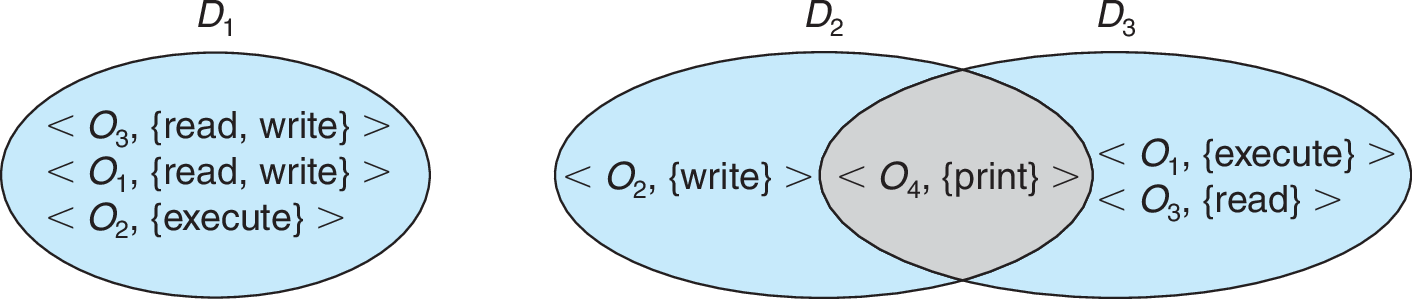
\includegraphics[width=8cm]{figs/04-14_01.pdf}
  \end{center}

\end{frame}


%---------------------------------------------------------------------
\begin{frame}
  \frametitle{Dominios de protección}

  Dominios de protección ¿cumplen principio de menores privilegios?
  
  \begin{itemize}
    \item Se necesita un {\bf mecanismo} de cambio de dominio
  \end{itemize}
  
  Modo dual monitor-usuario es un ejemplo de cambio de dominio (muy básico)
  \begin{itemize}
    \item Sistemas multiusuario requieren más granularidad de privilegios
    \item Dominios pueden ser procesos, usuario, o procedimientos
  \end{itemize}

\end{frame}

%---------------------------------------------------------------------
\begin{frame}
  \frametitle{Dominios de protección: UNIX}

  UNIX implementa dominios de protección como usuarios.
  \begin{itemize}
    \item Cambiar de domino implica cambiar de usuario
    \item Implementación a través del sistema de archivos
    \item Cada archivo $F$ posee un propietario ({\em owner}) y un {\em domain bit}, 
          también conocido como {\bf setuid bit}
      \begin{itemize}
        \item Si {\bf setuid == 1}, owner$(F)==A$, y $B$ ejecuta $F$, entonces $F$ se ejecuta como el usuario $A$
        \item Si {\bf setuid == 0}, owner$(F)==A$, y $B$ ejecuta $F$, entonces $F$ se ejecuta como el usuario $B$
        \item Cambio temporal de {\em userID}
        \item ¿Para qué puede servir esto?
      \end{itemize}
  \end{itemize}
\end{frame}

%---------------------------------------------------------------------
\begin{frame}
  \frametitle{Dominios de protección: MULTICS}

  MULTICS implementa dominios como anillos.

  Procesos en dominios internos tienen más privilegios que los externos.

  \begin{center}
    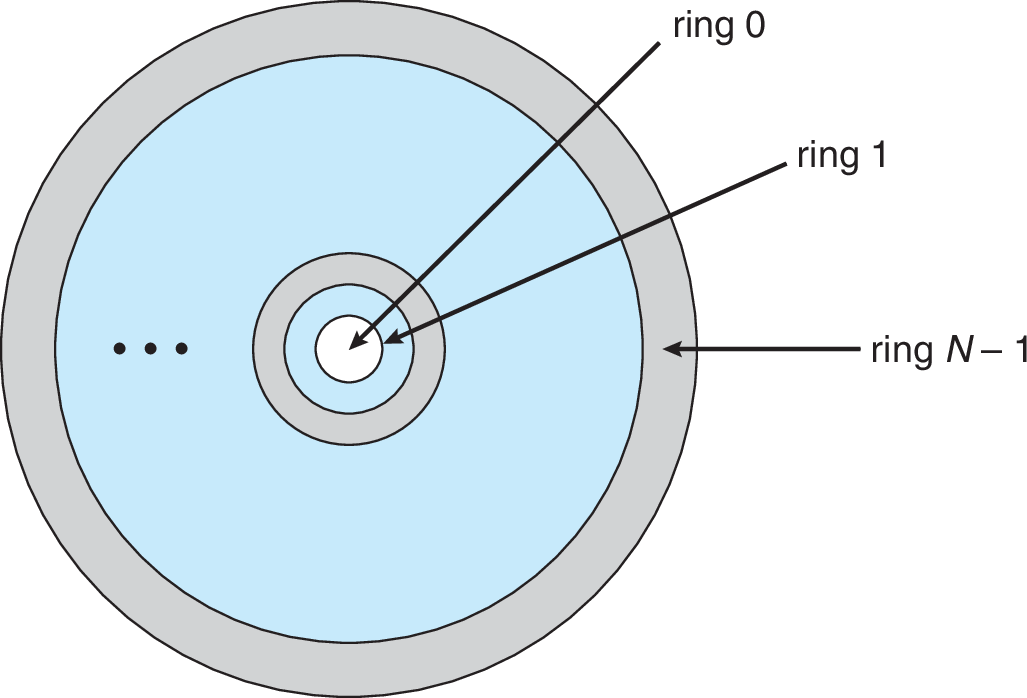
\includegraphics[width=8cm]{figs/04-14_02.pdf}
  \end{center}

\end{frame}

%---------------------------------------------------------------------
\begin{frame}
  \frametitle{Matrices de acceso}

  Filas representan dominios. Columnas representan objetos.


  \begin{center}
    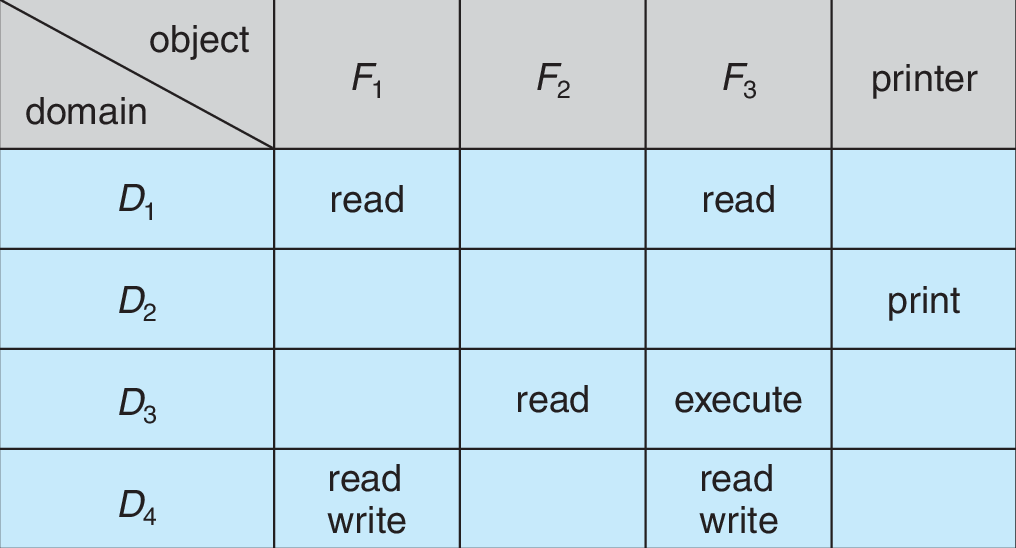
\includegraphics[width=8cm]{figs/04-14_03.pdf}
  \end{center}

  Objeto nuevo implica columna nueva, administrada por su {\em owner}.
  
  
\end{frame}

%---------------------------------------------------------------------
\begin{frame}
  \frametitle{Matrices de acceso: {\tt switch}}

  {\tt switch} permite cambiar de dominio

  \begin{center}
    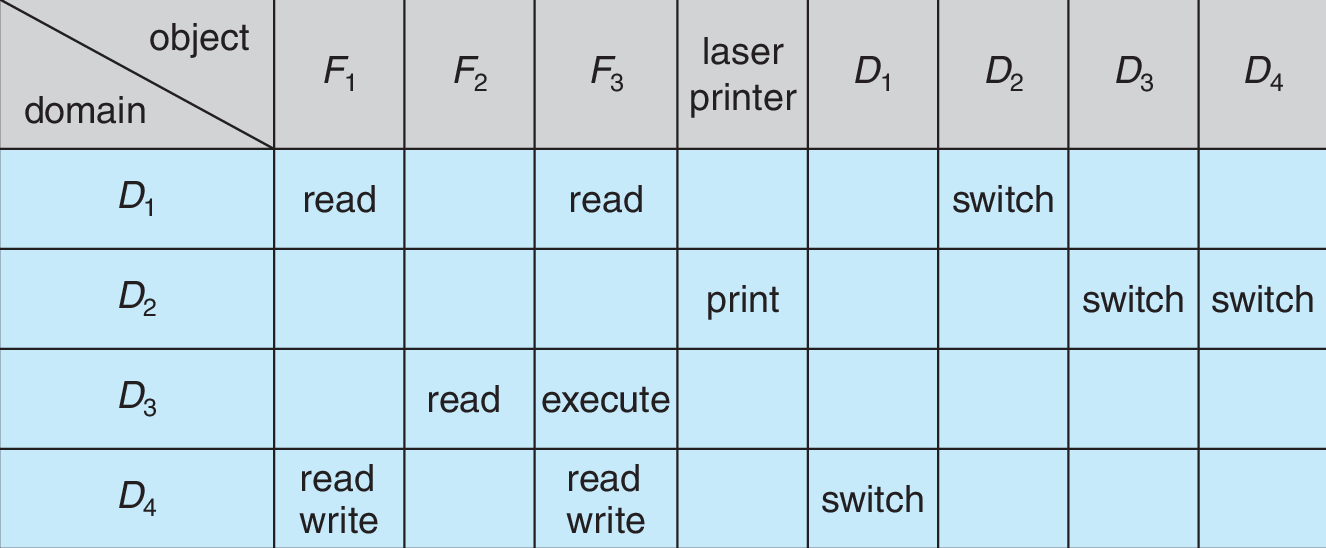
\includegraphics[width=8cm]{figs/04-14_04.pdf}
  \end{center}
  
  {\tt switch(i,j)} permite cambiar de dominio {\tt i} a {\tt j}
  
\end{frame}


%---------------------------------------------------------------------
\begin{frame}
  \frametitle{Matrices de acceso: {\tt copy}}

  Algunos dominios permiten copiar ({\tt *}) atributos.


  \begin{center}
    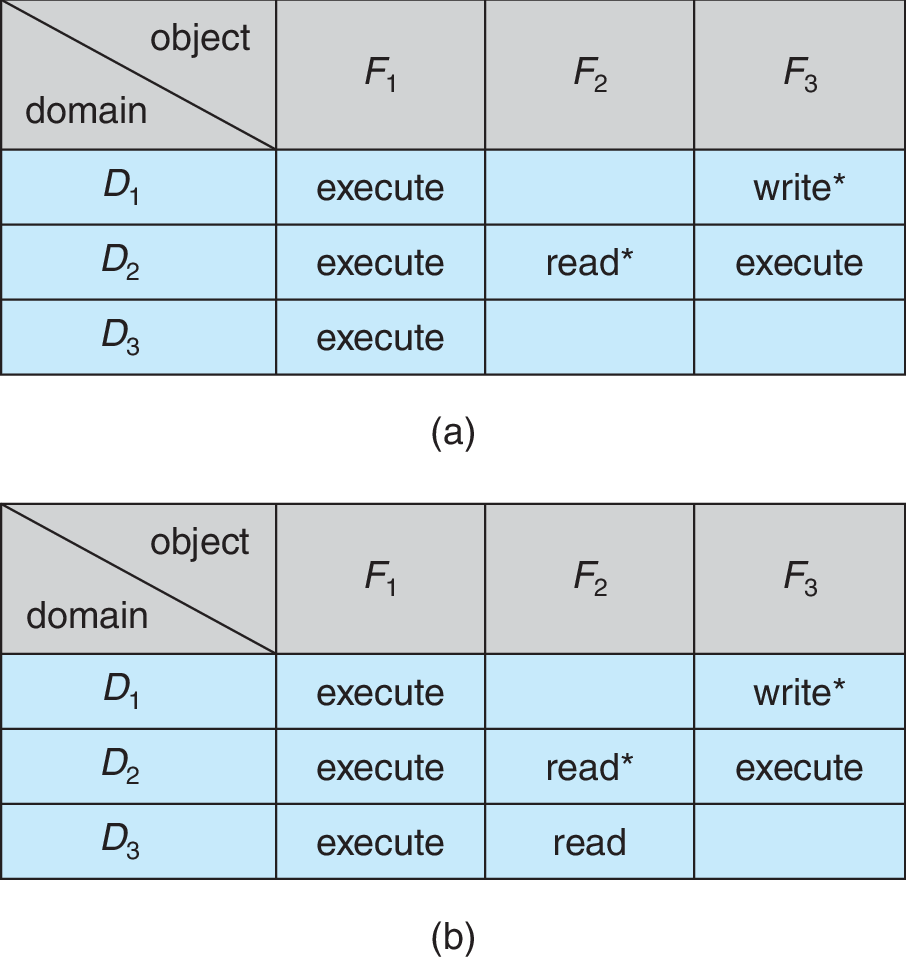
\includegraphics[width=4cm]{figs/04-14_05.pdf}
  \end{center}

  Variantes:
  \begin{itemize}
    \item copy
    \item transfer
    \item limited copy
  \end{itemize}
  
\end{frame}

%---------------------------------------------------------------------
\begin{frame}
  \frametitle{Matrices de acceso: {\tt owner}}

  Atributo de {\tt owner} permite agregar y modificar atributos.


  \begin{center}
    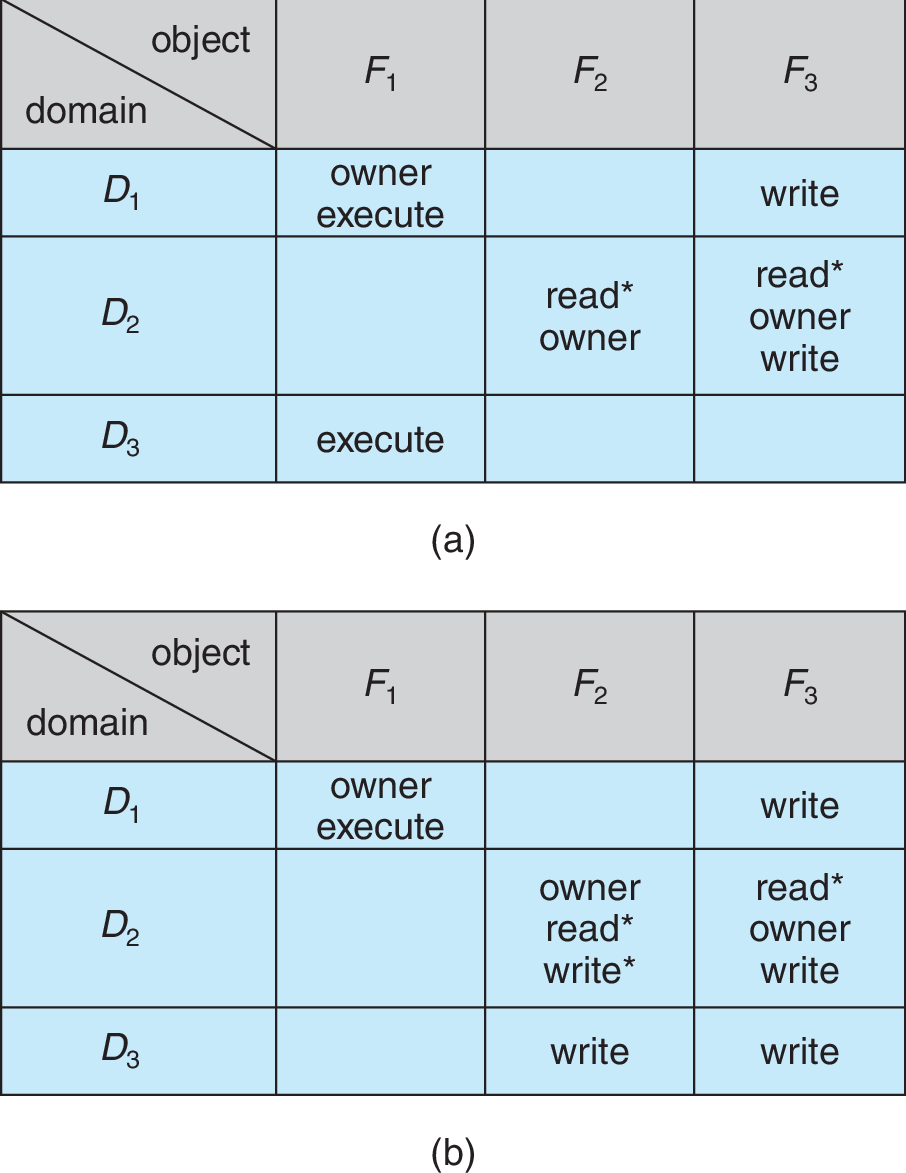
\includegraphics[width=4cm]{figs/04-14_06.pdf}
  \end{center}

  
\end{frame}




%---------------------------------------------------------------------
\section{Seguridad}

%---------------------------------------------------------------------
\begin{frame}
  \frametitle{Seguridad}
  No basta con protegerse de los ataques internos... también hay ataques {\bf externos}.
  
  \begin{block}{Sistema seguro}
    Un sistema es seguro si garantiza que sus recursos son accedidos y utilizados
    bajo toda circunstancia.
  \end{block}

  \begin{itemize}
    \item {\bf Intruso}, {\bf cracker}. Personaje que intenta romper la seguridad.
    \item {\bf Threat}, {\bf amenaza}. Potencialidad de violación a la seguridad. Ej: descubrimiento de vulnerabilidad
    \item {\bf Ataque}. Intento de romper la seguridad.
  \end{itemize}

\end{frame}
%---------------------------------------------------------------------
\begin{frame}
  \frametitle{Seguridad: tipos de ataques}
  \begin{itemize}
    \item {\bf Brecha de confidencialidad}. Lectura de datos secretos.
    \item {\bf Brecha de integridad}. Modificación de datos.
    \item {\bf Brecha de disponibilidad}. Ej: web defacement
    \item {\bf TOS. Theft of service}. Uso no autorizado de recursos.
    \item {\bf DOS. Denial of service}. Evitar uso del sistema.
  \end{itemize}

\end{frame}
%---------------------------------------------------------------------
\begin{frame}
  \frametitle{{\bf Masquerading}, {\bf man-in-the-middle}}

  \begin{center}
    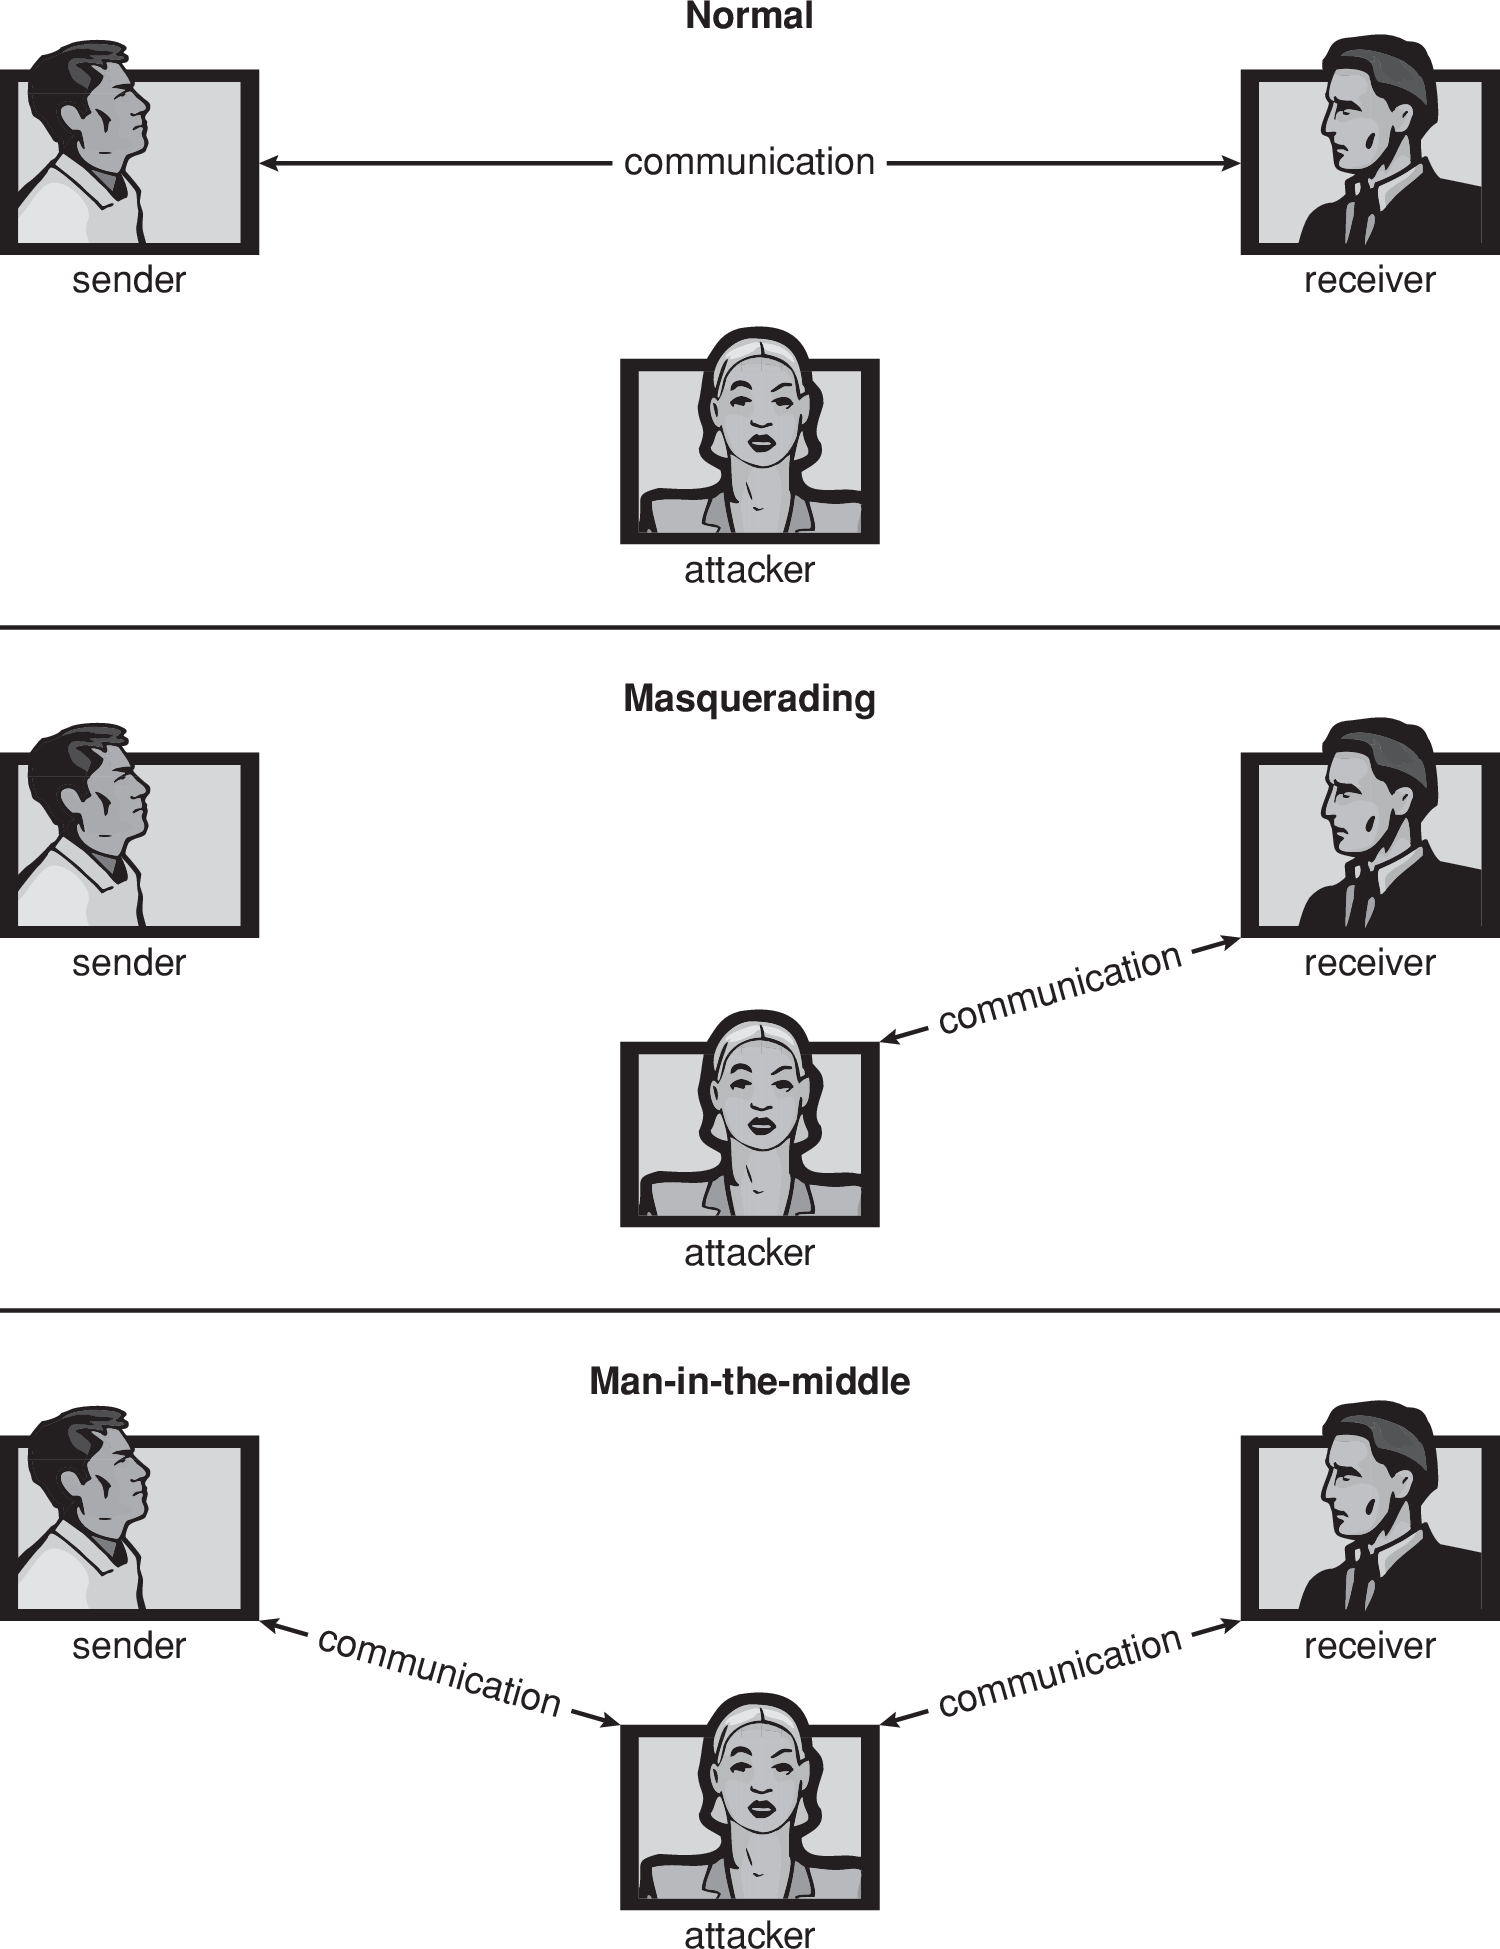
\includegraphics[width=5cm]{figs/04-15_01.pdf}
  \end{center}

\end{frame}

%---------------------------------------------------------------------
\begin{frame}
  \frametitle{Niveles de seguridad}

  \begin{itemize}
    \item {\bf Nivel físico}. Proteger acceso físico.
    \item {\bf Nivel humano}. Social engineering, phishing.
    \item {\bf Nivel de SO}. Accidental DOS. Stack overflow.
    \item {\bf Nivel de red}. Intercepción de comunicación.
  \end{itemize}

\end{frame}
%---------------------------------------------------------------------
\begin{frame}
  \frametitle{Programas maliciosos}

  \begin{itemize}
    \item {\bf Trojan horse}. Login emulator. Spyware.
    \item {\bf Trap door}. Creado por el diseñador/programador/compilador.
    \item {\bf Logic bomb}. Código que se activa solo bajo ciertas circunstancia
    \item {\bf Stack/buffer overflow}. Aprovechan {\em bug}s del código.
      \begin{enumerate}
        \item Provocar {\em overflow} de {\em input}, {\em linea de comando}, {\em buffer},
              hasta hacer que quede código en el {\em stack}.
        \item Sobreescribir la dirección de retorno con la dirección del siguiente código.
        \item Reemplazar el código en el lugar apuntado, con código propio
      \end{enumerate}
  \end{itemize}
  
\end{frame}
%---------------------------------------------------------------------
\begin{frame}[fragile]
  \frametitle{Buffer overflow}
  
\begin{minted}[mathescape,numbersep=5pt,gobble=0,frame=lines,framesep=2mm,fontsize=\small,linenos=true]{c}
#include <stdio.h>
#define BUFFER SIZE 256
int main(int argc, char *argv[]) {
  char buffer[BUFFER SIZE];
  if (argc < 2)
    return -1;
  else { 
    strcpy(buffer,argv[1]); 
    return 0;
  }
}

\end{minted}
  
\end{frame}
%---------------------------------------------------------------------
\begin{frame}
  \frametitle{Buffer overflow}

  Stack frame

  \begin{center}
    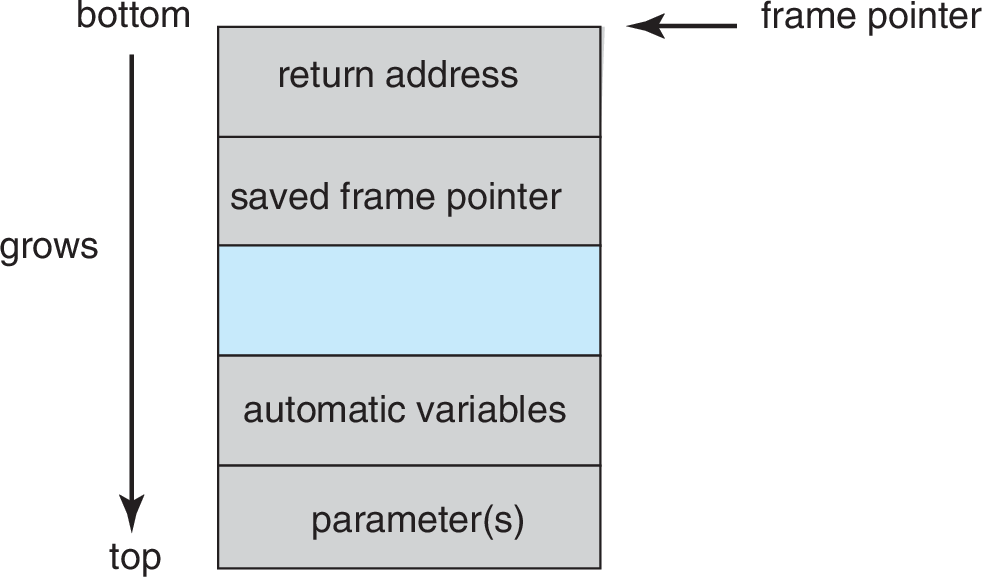
\includegraphics[width=7cm]{figs/04-15_03.pdf}
  \end{center}

\end{frame}
%---------------------------------------------------------------------
\begin{frame}[fragile]
  \frametitle{Buffer overflow}

  ¿Qué hace este código?

\begin{minted}[mathescape,numbersep=5pt,gobble=0,frame=lines,framesep=2mm,fontsize=\small,linenos=true]{c}
#include <stdio.h>

int main(int argc, char *argv[]) {
  execvp("\bin\sh","\bin \sh", NULL);
  return 0;
}

\end{minted}

\end{frame}
%---------------------------------------------------------------------
\begin{frame}
  \frametitle{Buffer overflow}

  Ataque intenta modificar el {\em stack frame}
  
  \begin{center}
    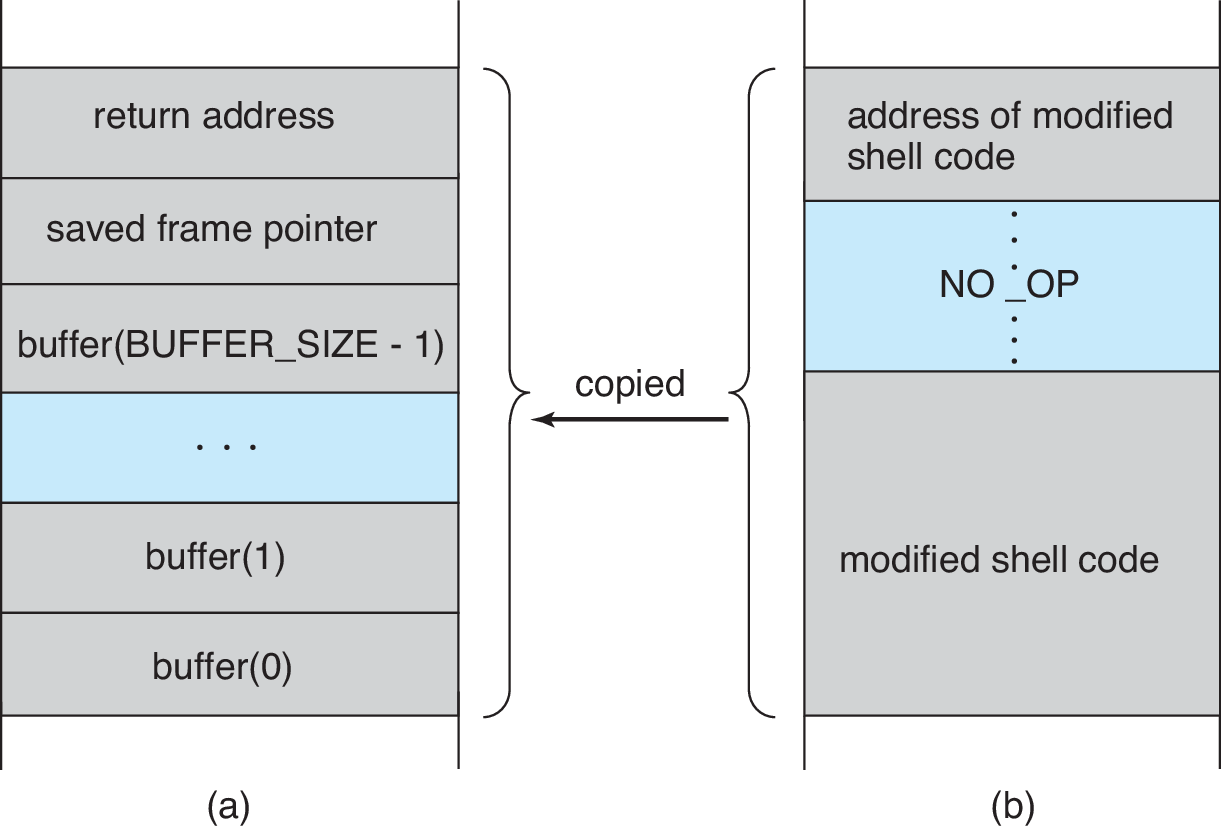
\includegraphics[width=7cm]{figs/04-15_04.pdf}
  \end{center}

  Ataque necesita conocer la dirección de {\tt buffer[0]}
  
  Al terminar, en lugar de ejecutar la {\tt return address}, ejecuta el código copiado.
\end{frame}

%---------------------------------------------------------------------
\begin{frame}
  \frametitle{Virus}

  Segmento de código agregar a código ``sano''. Al ejecutar el código infectado, se ejecuta 
  el código del virus.

  \begin{center}
    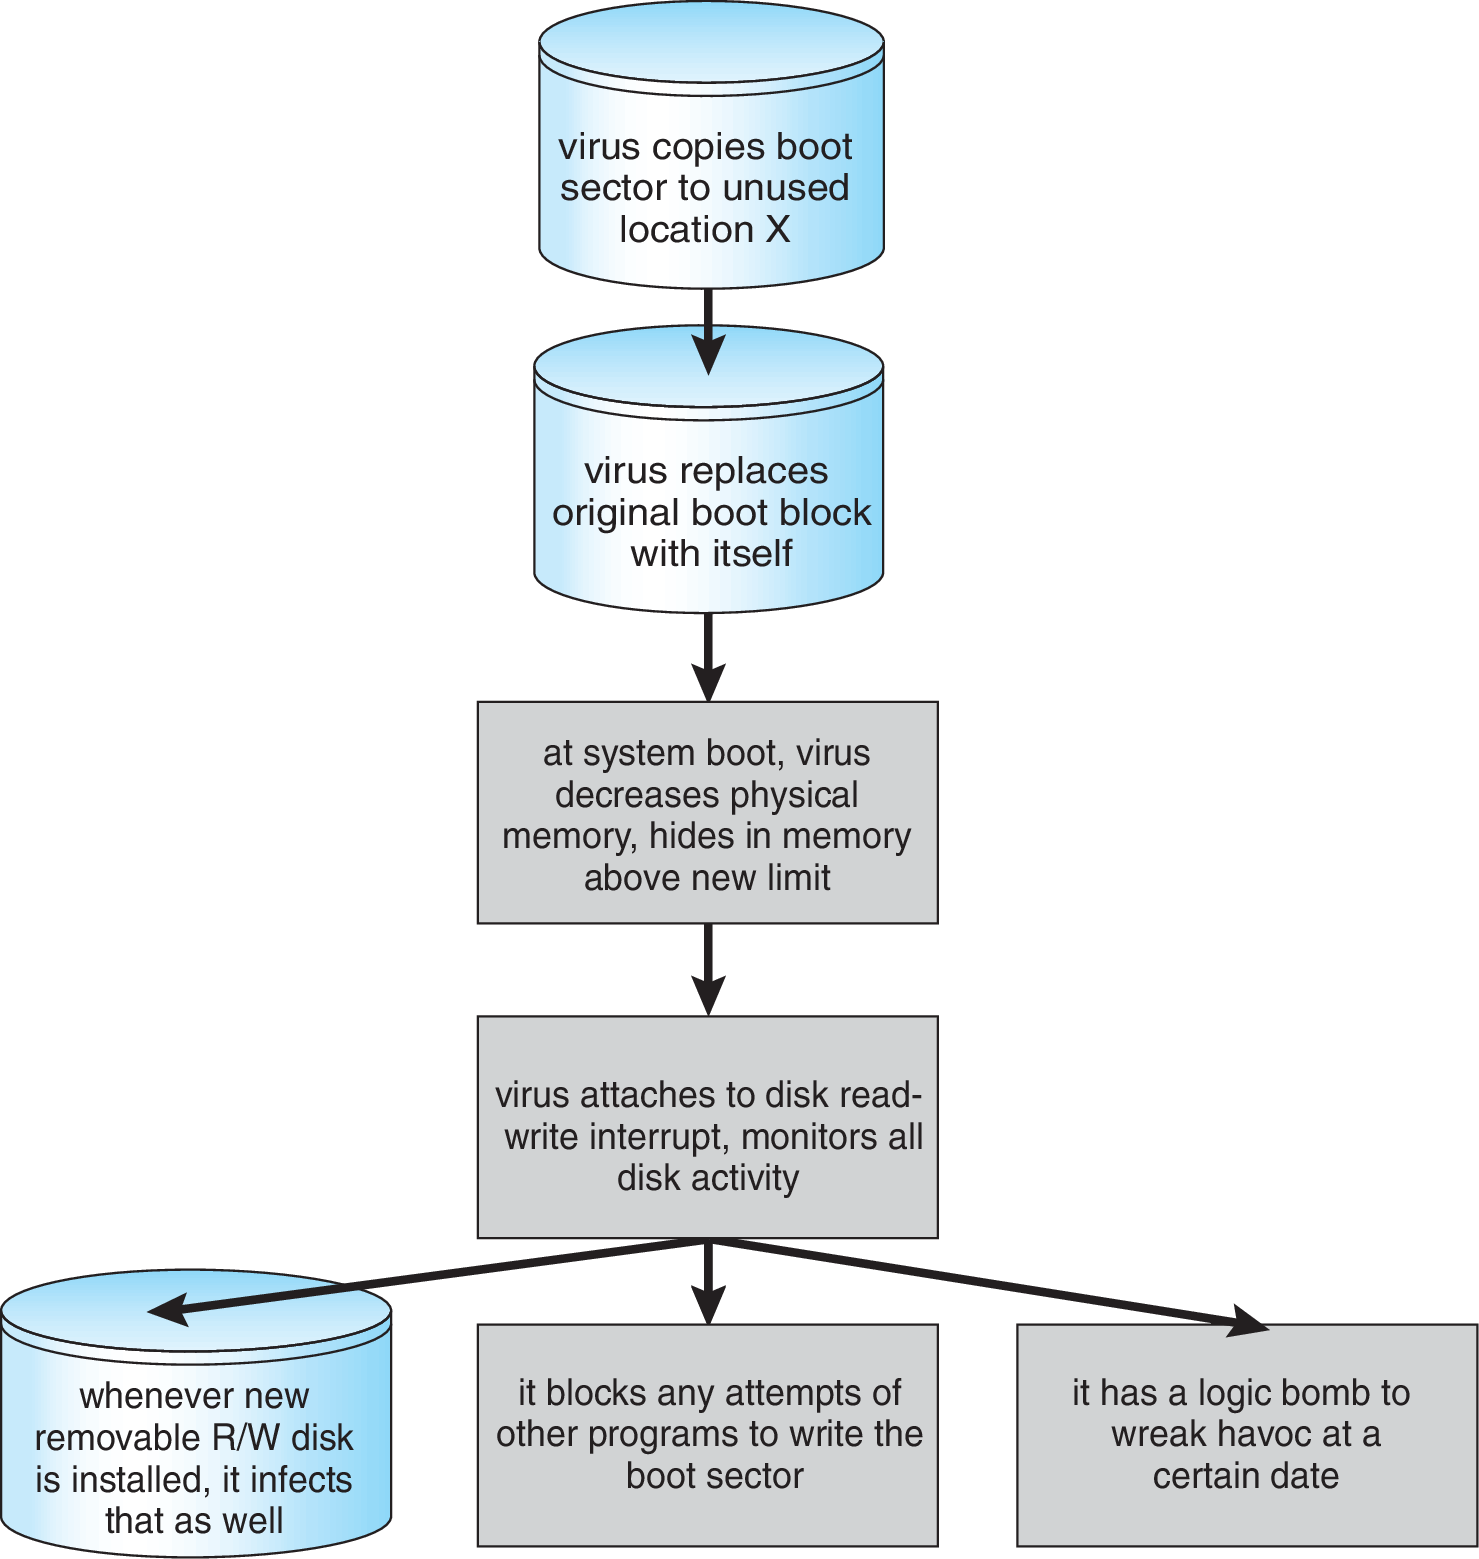
\includegraphics[width=6cm]{figs/04-15_05.pdf}
  \end{center}
  
  
\end{frame}
%---------------------------------------------------------------------
\begin{frame}
  \frametitle{Worms}

  Código que aprovecha vulnerabilidades de sistema y red para autoreplicarse.
  
  \begin{center}
    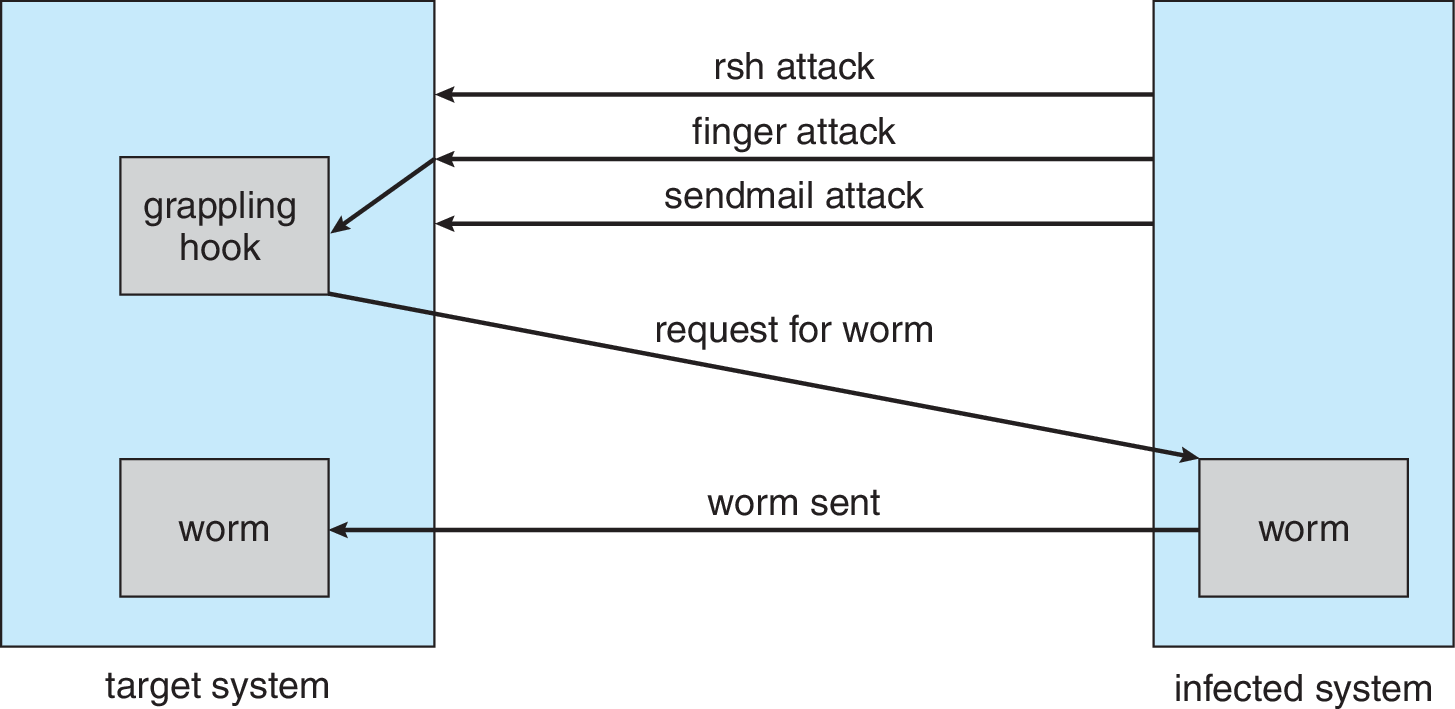
\includegraphics[width=8cm]{figs/04-15_06.pdf}
  \end{center}
  
  
\end{frame}



%---------------------------------------------------------------------
\end{document}